\chapter{Further Applications}\label{chap:extension}
\todo{chapter intro}


\section{Covid-19 Period (February-April 2020)}

the first ten weeks for in-sample and the last three weeks for out-of-sample

\begin{table}[ht]
\centering
\small
\renewcommand{\arraystretch}{1.3} % Increases row height
\setlength{\tabcolsep}{10pt} % Increases column separation
\resizebox{\textwidth}{!}{%
\begin{tabular}{|c|l|c|}
\hline
\textbf{Purpose}       & \multicolumn{1}{c|}{\textbf{Timeframe}} & \textbf{Number of transactions} \\ \hline
Panel C: Total         & February 3 - April 30, 2020           & 786,598                      \\ \hline
Panel D: In-sample     & February 3 - April 11, 2020            & 660,487 (84\% of total sample) \\ \hline
Panel D: Out-of-sample & April 12 - April 30, 2020          & 126,111 (16\% of total sample)   \\ \hline
\end{tabular}%
}
\caption{Summary of Database: IBM traded on NYSE (February-April 2020).}
\label{tab:table-12}
\end{table}




\begin{table}[h]
  \centering
  \setlength{\tabcolsep}{4pt} 
  \resizebox{\textwidth}{!}{%
    \begin{tabular}{@{} r *{14}{r} @{}}
      \toprule
      \textbf{Category}      & 1    & 2       & 3       & 4       & 5       & 6       & 7       & 8       & 9       & 10   
      & 11      & 12      & 13      & 14      \\
      
      \textbf{Price Changes}   & <–6  & [–6,–5) & [–5,–4) & [–4,–3) & [–3,–2) & [–2,–1) & [–1,0)  & [0,1)   & [1,2)   & [2,3)   & [3,4)   & [4,5)   & [5,6)   & \geq6     \\
    
      \textbf{Percentage} & 2.98\% & 0.57\% & 2.04\% & 4.14\% & 2.39\% & 9.58\% & 5.71\% & 51.28\% & 9.28\% & 2.37\% & 4.04\% & 1.96\% & 0.55\% & 3.08\%\\
      \bottomrule
    \end{tabular}%
  }
  \caption{Frequencies of Partition (February-April 2020).}
  \label{tab:table-14}
\end{table}



\begin{table}[htbp]
    \centering
    \vspace{0.5em}
    \begin{tabular}{crrl}
        \toprule
        Df & $\chi^2$ & Pr($>$$\chi^2$) \\
        \midrule
         2 & 2835.2 & $<$ 2.2e-16 *** \\ 
         \bottomrule
        \multicolumn{3}{l}{$^{***}p < 0.001$; $^{**}p < 0.01$; $^{*}p < 0.05$}
    \end{tabular}
        \caption{Sequence of Trade: Linear Hypothesis Test (February-April 2020).}
    \label{tab:table-18}
\end{table}


\begin{table}[H]
\centering
\begin{tabular}{lrr}
\toprule
 & \multicolumn{1}{c}{\$Volume} & \multicolumn{1}{r}{Impact} \\
\midrule
\multicolumn{3}{l}{\textbf{Increasing price sequence (1/1/1)}} \\
\addlinespace[0.5ex]
\multicolumn{3}{l}{\emph{Price impact in ticks}} \\
E$[Z_k]$             &  500   &  $0.0802$ \\
$\Delta E[Z_k]$      & 1{,}000   &   $0.1664$ \\
$\Delta E[Z_k]$      & 1{,}500   &   $0.3337$ \\
$\Delta E[Z_k]$      & 2{,}000   &   $0.5027$ \\
$\Delta E[Z_k]$      & 2{,}500   &   $0.6742$ \\
$\Delta E[Z_k]$      & 5{,}500   &   $1.7823$ \\
\addlinespace[1ex]
\multicolumn{3}{l}{\emph{Price impact in percent}} \\
E$[Z_k]$             &  500   &  $0.0006$ \\
$\Delta E[Z_k]$      & 1{,}000   &   $0.0013$ \\
$\Delta E[Z_k]$      & 1{,}500   &   $0.0027$ \\
$\Delta E[Z_k]$      & 2{,}000   &   $0.0040$ \\
$\Delta E[Z_k]$      & 2{,}500   &   $0.0054$ \\
$\Delta E[Z_k]$      & 5{,}500   &   $0.0143$ \\
\midrule
\multicolumn{3}{l}{\textbf{Constant price sequence (0/0/0)}} \\
\addlinespace[0.5ex]
\multicolumn{3}{l}{\emph{Price impact in ticks}} \\
E$[Z_k]$             &  500   &  $-0.0144$ \\
$\Delta E[Z_k]$      & 1{,}000   &   $0.1663$ \\
$\Delta E[Z_k]$      & 1{,}500   &   $0.3330$ \\
$\Delta E[Z_k]$      & 2{,}000   &   $0.5009$ \\
$\Delta E[Z_k]$      & 2{,}500   &   $0.6709$ \\
$\Delta E[Z_k]$      & 5{,}500   &   $1.7655$ \\
\addlinespace[1ex]
\multicolumn{3}{l}{\emph{Price impact in percent}} \\
E$[Z_k]$             &  500   &  $-0.0001$ \\
$\Delta E[Z_k]$      & 1{,}000   &   $0.0013$ \\
$\Delta E[Z_k]$      & 1{,}500   &   $0.0027$ \\
$\Delta E[Z_k]$      & 2{,}000   &   $0.0040$ \\
$\Delta E[Z_k]$      & 2{,}500   &   $0.0054$ \\
$\Delta E[Z_k]$      & 5{,}500   &   $0.0142$ \\
\bottomrule
\end{tabular}

\caption{Impact of Trade Size (February-April 2020).}
\label{tab:table-19}
\end{table}




\begin{table}[H]
\centering
\begin{tabular}{@{}lcc@{}}
\toprule
\multicolumn{1}{c}{Metric} & \multicolumn{1}{l}{\textbf{\% Accuracy}} & \multicolumn{1}{l}{\textbf{Hand-Till Multiclass AUC}} \\ \midrule
\textbf{In-sample}         & 51.8 \%                                 & 0.6133                                                \\
\textbf{Out-of-sample}     & 48.6 \%                                 & 0.6088                                                \\ \bottomrule
\end{tabular}
\caption{Forecasts Evaluation for In- and Out-of-sample (February-April 2020).}
\label{tab:table-20}
\end{table}



\begin{figure}[H]
    \centering
    \resizebox{0.85\textwidth}{!}{%
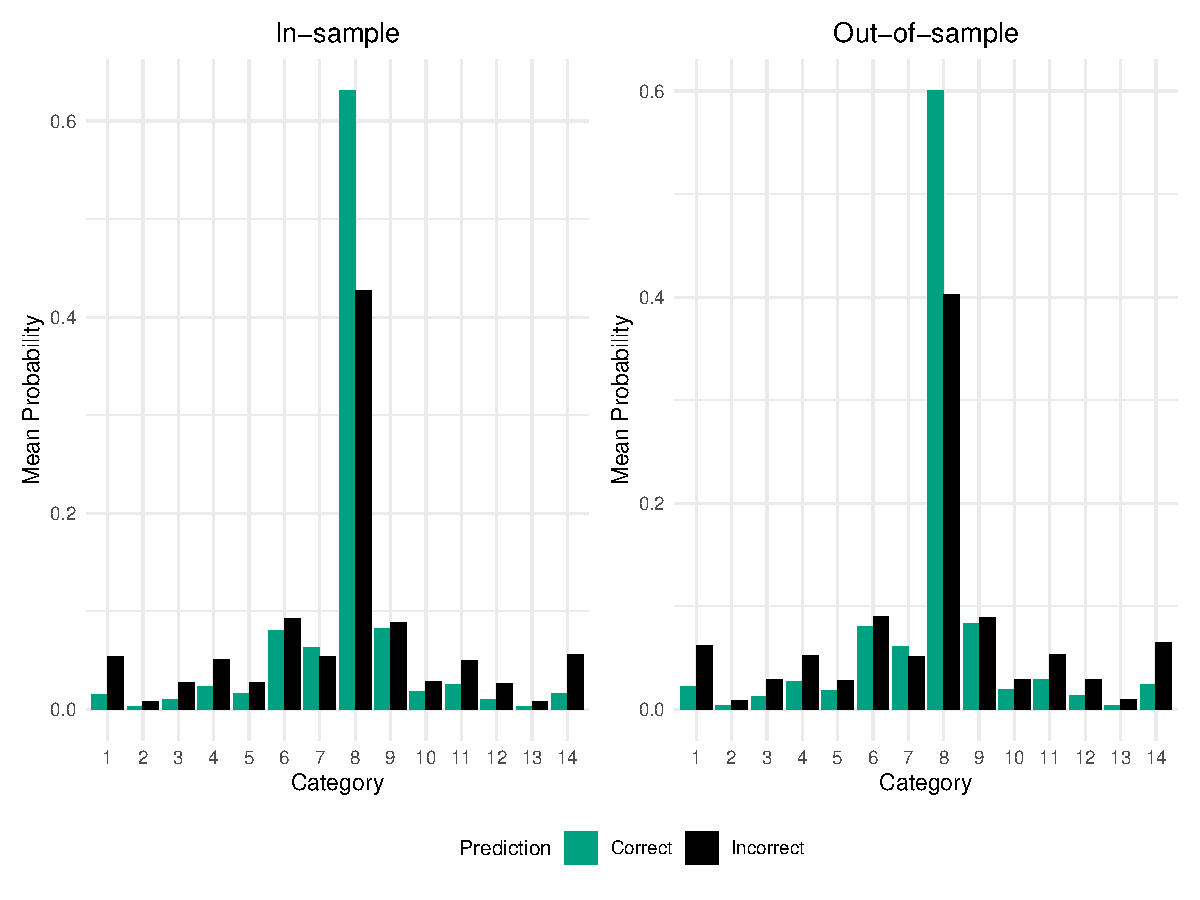
\includegraphics{figures/covid 19 period/overfitting_compare_covid.pdf}}
    \caption{Mean Probability by Prediction Class of In- and Out-of-sample (February-April 2020).}
    \label{fig:figure-6}
\end{figure}








\section{2008 Financial Crisis (September-October 2008)}

\begin{table}[ht]
\centering
\small
\renewcommand{\arraystretch}{1.3} % Increases row height
\setlength{\tabcolsep}{10pt} % Increases column separation
\resizebox{\textwidth}{!}{%
\begin{tabular}{|c|l|c|}
\hline
\textbf{Purpose}       & \multicolumn{1}{c|}{\textbf{Timeframe}} & \textbf{Number of transactions} \\ \hline
Panel E: Total         & September 2 - October 31, 2008          & 508,714                     \\ \hline
Panel F: In-sample     & September 2 - October 19, 2008            & 390,540 (77\% of total sample) \\ \hline
Panel F: Out-of-sample & October 20 - October 31, 2008          & 118,174 (23\% of total sample)   \\ \hline
\end{tabular}%
}
\caption{Summary of Database: IBM traded on NYSE (September-October 2008).}
\label{tab:table-21}
\end{table}



\begin{table}[H]
  \centering
  \setlength{\tabcolsep}{4pt} 
  \resizebox{\textwidth}{!}{%
    \begin{tabular}{@{} r *{14}{r} @{}}
      \toprule
      \textbf{Category}      & 1    & 2       & 3       & 4       & 5       & 6       & 7       & 8       & 9       & 10   
      & 11      & 12      & 13      & 14      \\
      
      \textbf{Price Changes}   & <–6  & [–6,–5) & [–5,–4) & [–4,–3) & [–3,–2) & [–2,–1) & [–1,0)  & [0,1)   & [1,2)   & [2,3)   & [3,4)   & [4,5)   & [5,6)   & \geq6     \\
    
      \textbf{Percentage} & 6.53\% & 0.79\% & 3.48\% & 4.95\% & 1.99\% & 9.98\% & 4.10\% & 40.81\% & 9.70\% & 1.98\% & 4.95\% & 3.50\% & 0.80\% & 6.44\%\\
      \bottomrule
    \end{tabular}%
  }
  \caption{Frequencies of Partition (September-October 2008).}
  \label{tab:table-23}
\end{table}

